\section{\ExercisePrefixEmbeddedC Eigenes Microcontroller-Projekt umsetzen \optional}

Nachdem du alle Ein- und Ausgabemöglichkeiten des Boards kennengelernt hast, besteht die Aufgabe in diesem Teil darin, ein beliebiges Programm, zum Beispiel ein Spiel, zu implementieren.
Du hast hierbei die freie Wahl, die folgenden Vorschläge sollen nur als Anregung dienen.
Um die Aufgabe leichter zu gestalten, empfiehlt es sich die beiliegende \lstinline{16FXlib} zu verwenden.
Die Dokumentation dazu findest du unter \url{http://echtzeitsysteme.github.io/tud-cpp-16FXlib/documentation/index.html}.

\subsection*{Vorschlag: Pong}
Zwei Gegner sollen je einen Balken (Rechteck) am linken oder rechten Rand des Spielfeldes mit den Schiebereglern steuern können, um einen Ball (ein Quadrat) im Spiel zu halten.
Erreicht der Ball den linken oder rechten Rand des Spielfelds, so bekommt der Spieler auf der anderen Seite einen Punkt und der Ball wird an seine Anfangsposition (die Mitte des Spielfelds) zurückversetzt.
Erreicht der Ball den oberen oder unteren Rand sowie einen der Balken der Spieler, so wird der Ball reflektiert - verlässt also niemals das Spielfeld.

Gewonnen hat der Spieler, der zuerst eine definierte Anzahl an Punkten erreicht.
Die aktuelle Punktzahl beider Spieler könnte auf der Siebensegmentanzeige ausgegeben werden.
\begin{center}
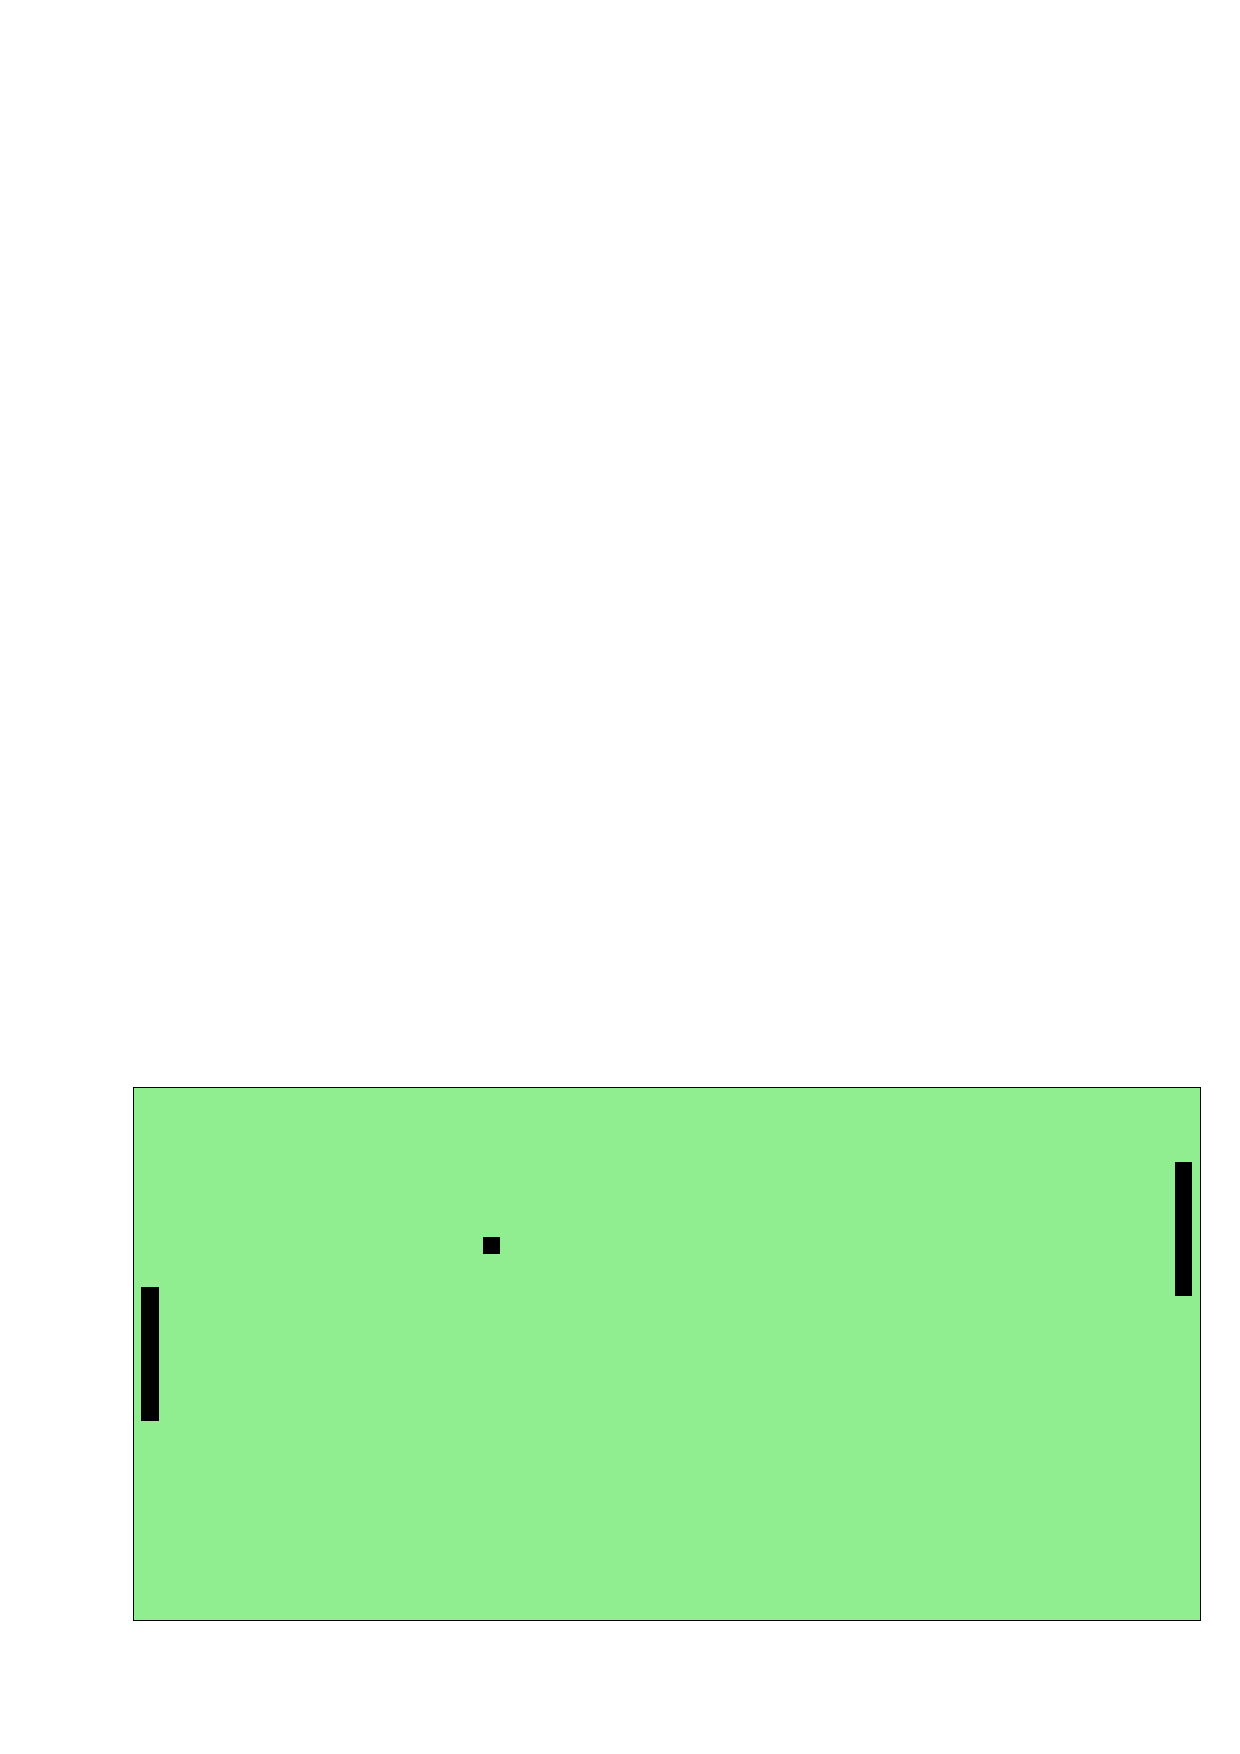
\includegraphics[scale=0.4]{05_c/figures/pong}
\end{center}



\subsection*{Vorschlag: Game of Life}
\glqq{}Game of Life\grqq{}\footnote{siehe auch \url{http://de.wikipedia.org/wiki/Conways_Spiel_des_Lebens}} besteht aus einem zweidimensionalen Spielfeld.
Jedes Feld steht für eine Zelle, die \textit{tot} (grün) oder \textit{lebendig} (schwarz) ist.
Jede Zelle hat acht Nachbarzellen, die ebenso tot oder lebendig sein können.
Zu Beginn gibt es eine vordefinierte Anfangsgeneration.
%
Durch festgelegte Regeln wird die nachfolgende Generation ermittelt:
\begin{itemize}
	\item Eine \textbf{lebende Zelle} \dots
	\begin{itemize}
		\item mit 1 oder 0 lebenden Nachbarn stirbt aus Einsamkeit.
		\item mit 4 oder mehr lebenden Nachbarn stirbt wegen Übervölkerung.
		\item mit 2 oder 3 lebenden Nachbarn bleibt am Leben.
	\end{itemize}
	\item Eine \textbf{tote Zelle} mit genau 3 lebenden Nachbarn wird in der nächsten Generation geboren werden, andernfalls bleibt sie tot.
\end{itemize}
%
Als Anfangsgeneration eignen sich zufällige Populationen oder eine der folgenden Figuren:
\begin{center}
	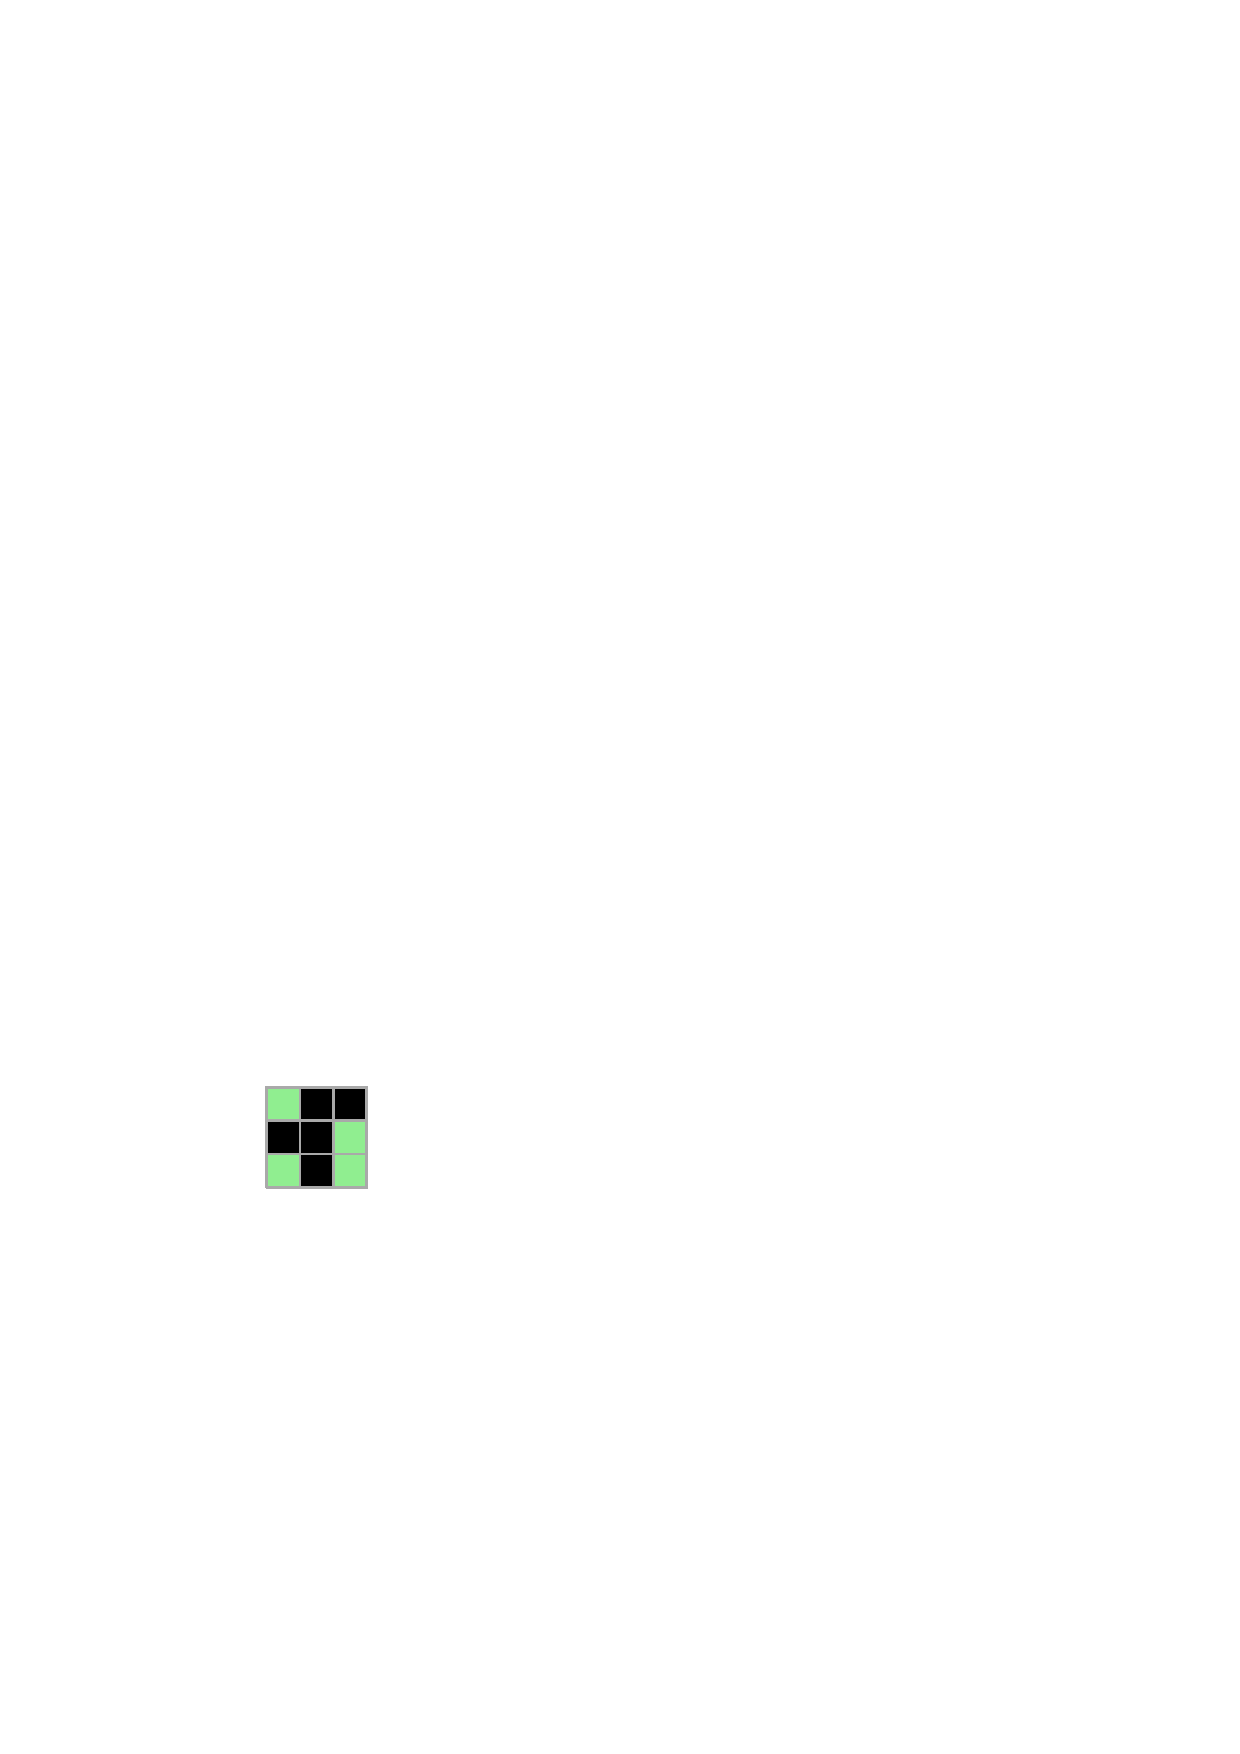
\includegraphics[scale=1]{05_c/figures/gol_init1}
	\hspace{5mm}
	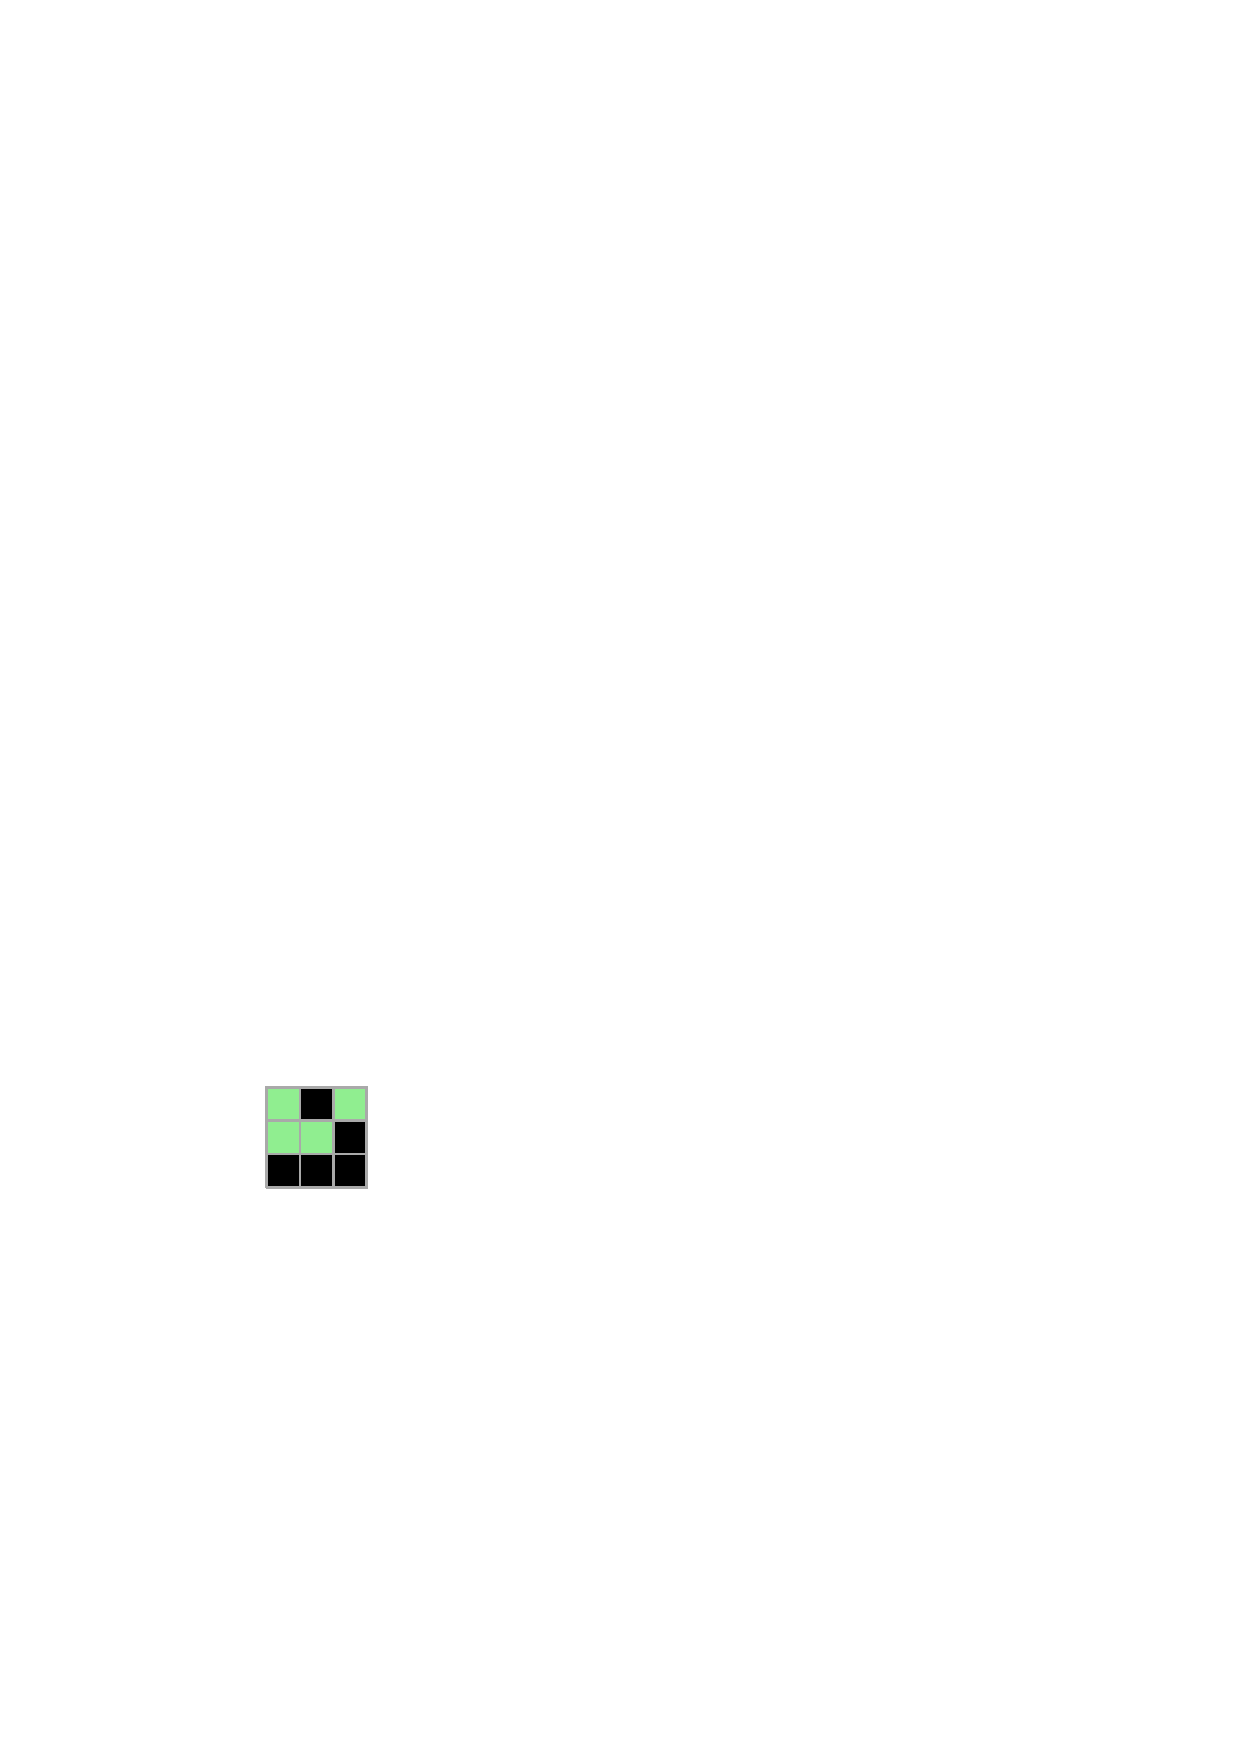
\includegraphics[scale=1]{05_c/figures/gol_init2}
	\hspace{5mm}
	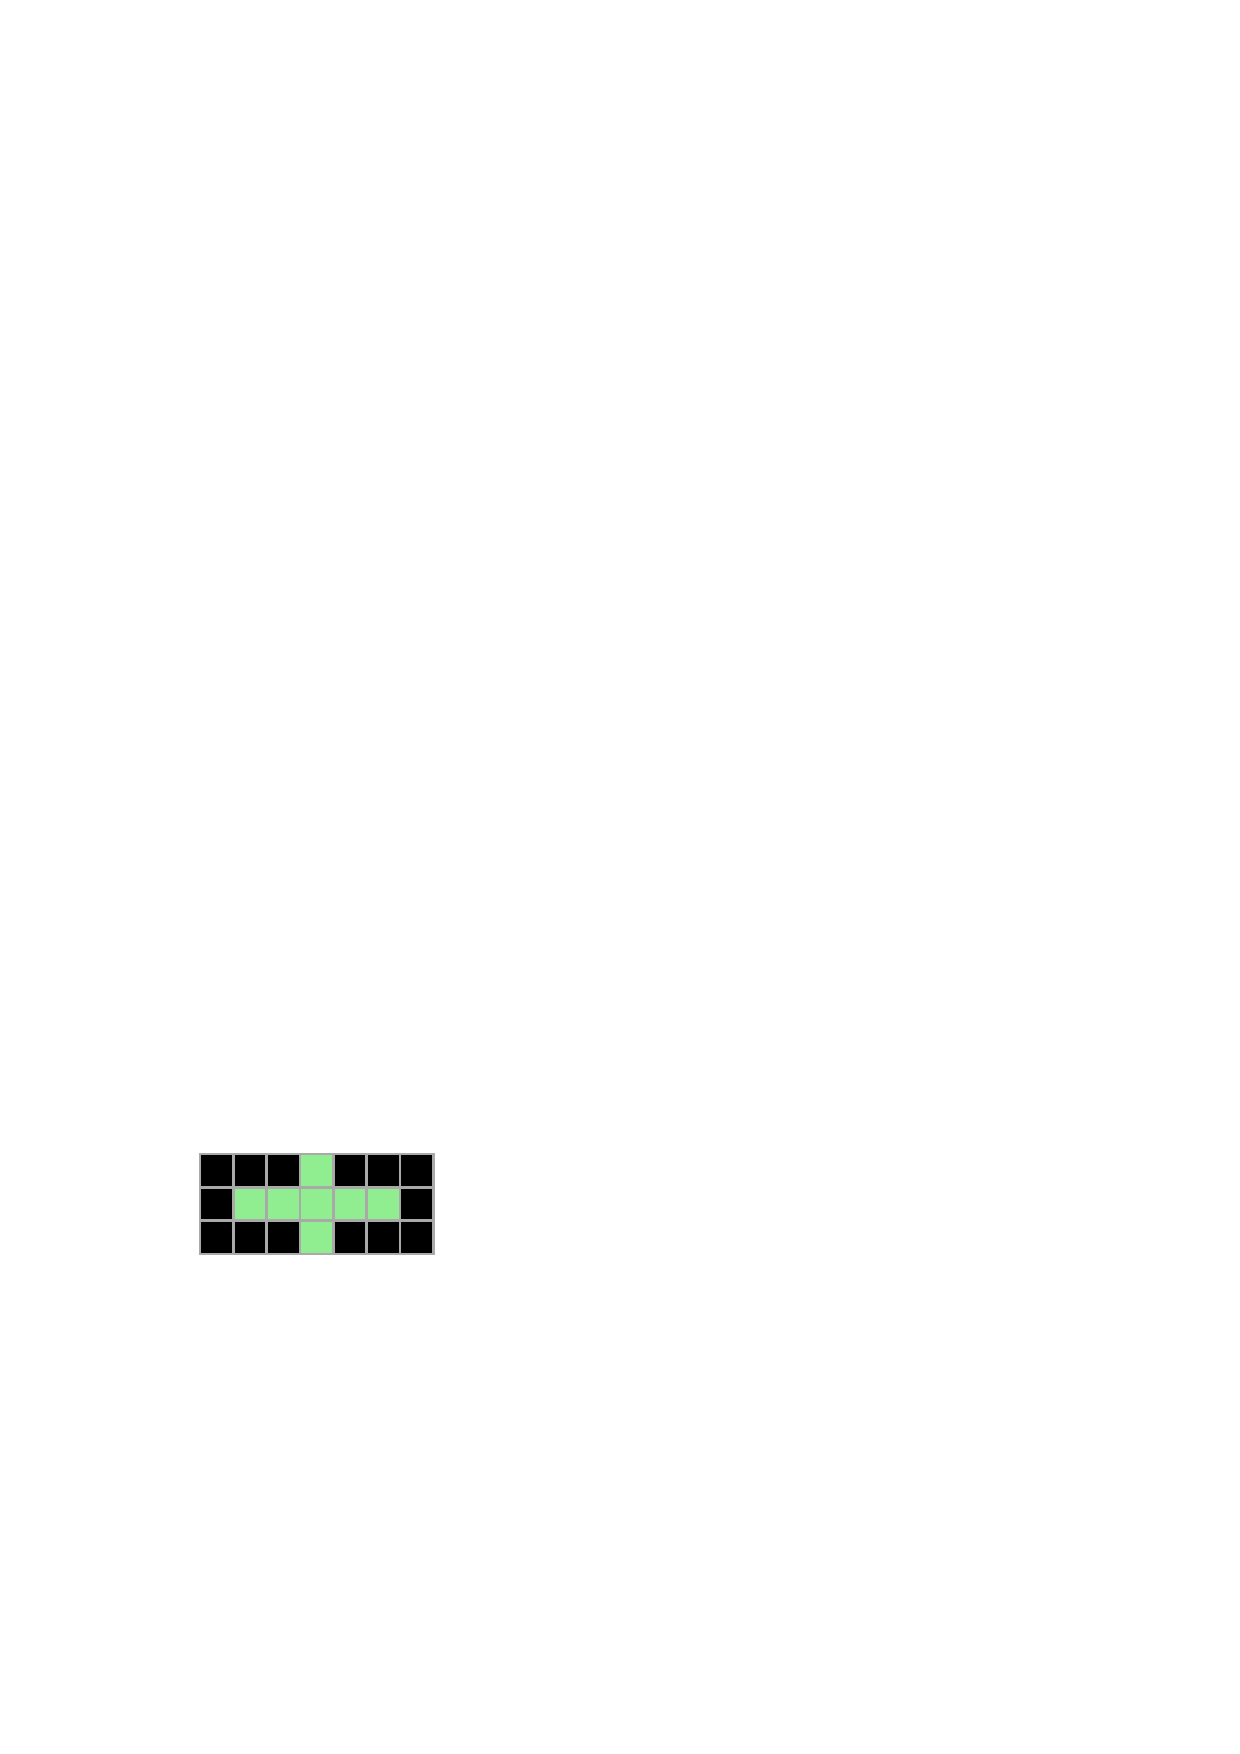
\includegraphics[scale=1]{05_c/figures/gol_init3}
\end{center}
%
\hints{
	\item Da das Spielfeld begrenzt ist, soll es torusförmig aufgebaut werden.
    Das heißt: Alles, was am unteren Rand des Spielfelds verschwindet, kommt oben wieder heraus -- das Gleiche gilt für den linken und rechten Rand. 
	\item Verwende als Spielfeld ein mehrdimensionales Array
	\item Ein weiteres mehrdimensionales Array bietet sich an, um die zukünftige Generation erzeugen zu können.
	\item Achte beim torusförmigen Feld unbedingt darauf, dass du nicht über die Grenzen des Spielfelds hinaus zugreifst!
    Das kann zu unvorhersehbarem und schwer zu debuggenen Verhalten des ganzen Displays führen!
}

\subsection*{Vorschlag: Regentropfen}

Das Touch-Display ist ein kleiner Teich;
wenn du eine Stelle mit dem Finger berührst, breitet sich von dort eine konzentrische Welle aus.
Die Geschwindigkeit der Welle kannst du zusätzlich abhängig machen vom ausgeübten Druck.


\subsection*{Weitere Vorschläge}
\RKi{Beispielbilder finden, CC4.0-kompatibel sind}
\begin{minipage}{.45\textwidth}
    \begin{center}Asteroids\\\vspace{4ex}
        %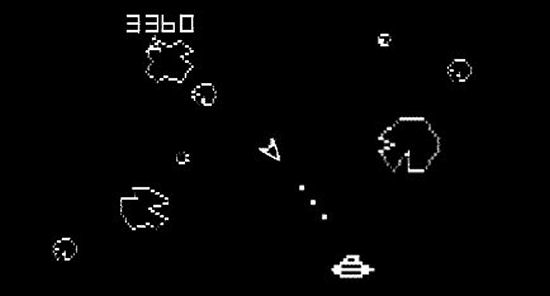
\includegraphics[width=.5\textwidth]{05_c/figures/img_asteroids.png}
    \end{center}
    \begin{center}Pacman\\\vspace{4ex}
        %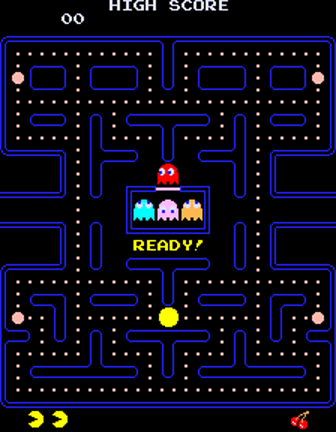
\includegraphics[width=.3\textwidth]{05_c/figures/img_pacman.png}
    \end{center}
    \begin{center}Labyrinth\\\vspace{4ex}
        %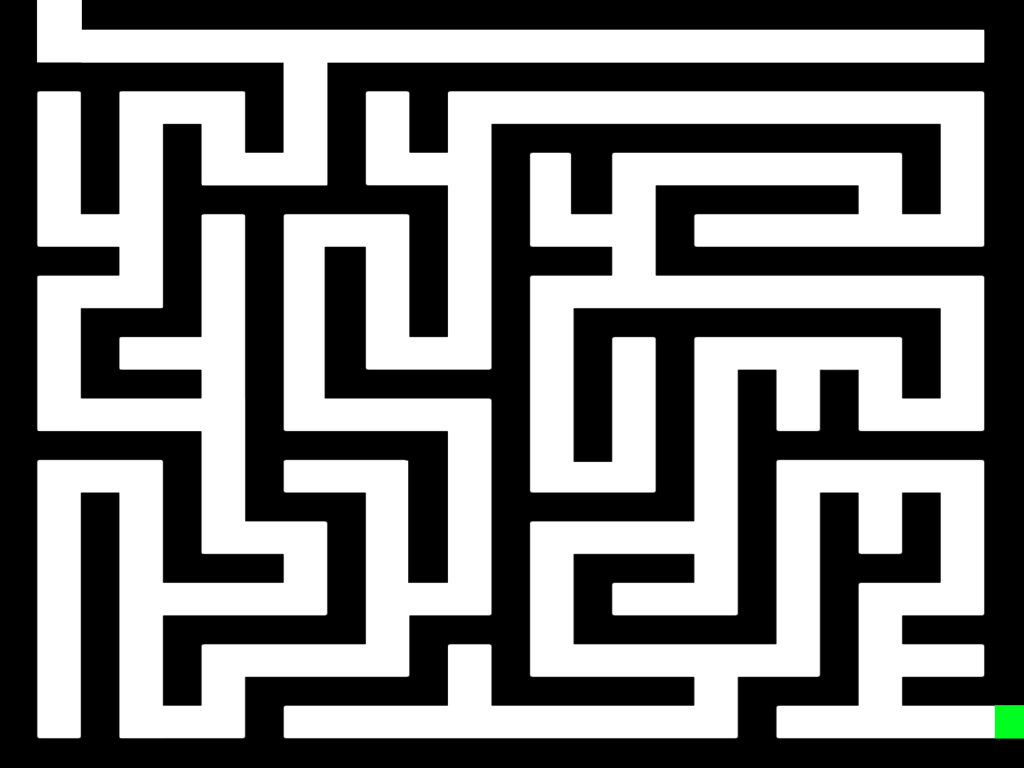
\includegraphics[width=.4\textwidth]{05_c/figures/img_maze.png}%
    \end{center}
\end{minipage}
\begin{minipage}{.45\textwidth}
	\begin{center}Ausweichspiele à la Hugo\\\vspace{4ex}
        %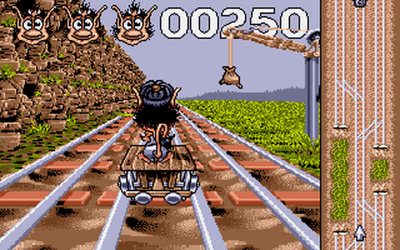
\includegraphics[width=.4\textwidth]{05_c/figures/img_hugo.png}
    \end{center}
	\begin{center}Moorhuhn\\\vspace{4ex}
        %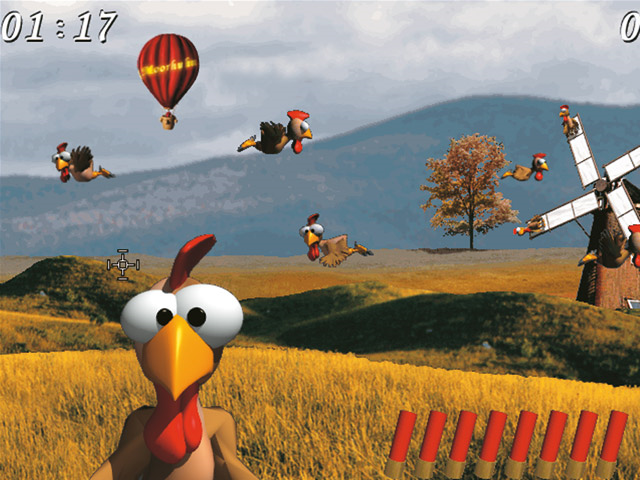
\includegraphics[width=.4\textwidth]{05_c/figures/img_moorhuhn.png}
    \end{center}
	\begin{center}Snake\\\vspace{4ex}%
       % 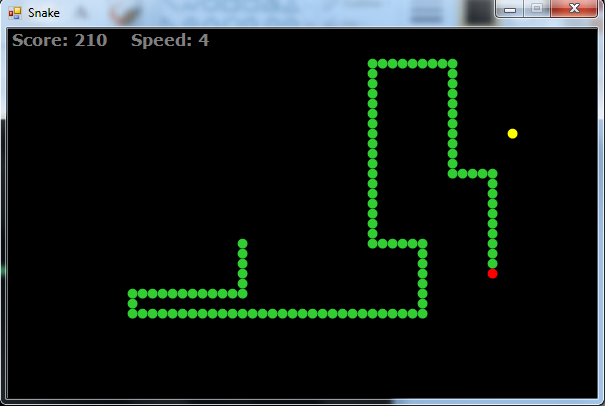
\includegraphics[width=.4\textwidth]{05_c/figures/img_snake.png}
    \end{center}
\end{minipage}


\hints{
	\item Möchte man ein Bild auf dem Board anzeigen, so empfiehlt es sich die einzelnen Pixeldaten in einem Array zu speichern.
	GIMP bietet hierfür die Möglichkeit eine Bilddatei als Header im \texttt{GIMP header image file format} zu exportieren.
	Da das Board nur zwei Farbwerte ermöglicht, sollte das Bild vor dem Exportieren über den Menüpunkt \textbf{Bild --> Modus} auf \textbf{indiziert \ldots} (Schwarz/Weiß-Palette (1-Bit)) gestellt werden.
	Anschließend kann man das \lstinline{header_data} Array verwenden, um auf die Bilddaten zuzugreifen.
}
